\documentclass{article}
\usepackage[utf8]{inputenc}
\usepackage{subcaption}
\usepackage{amsmath}
\usepackage{amssymb}
\usepackage{hyperref}
\usepackage{titlesec}
\usepackage{xcolor}
\usepackage{fancyhdr}
\usepackage{graphicx}
\usepackage{multirow}
\usepackage[rightcaption]{sidecap}
\usepackage{verbatim}
\usepackage [ a4paper , hmargin =1.2 in , bottom =1.5 in ] { geometry }
\hypersetup{
    colorlinks=true,
    linkcolor=blue,
    filecolor=magenta,      
    urlcolor=cyan,
}


% Add header and footer code here
\pagestyle{fancy}
\lhead{Minesweeper Cricket}
\rhead{Kavin Arvind (22B1019)}
\fancyfoot[C]{\thepage}

\begin{document}

% preamble
\thispagestyle{empty}
\title{Minesweeper Cricket}
\author{Kavin Arvind (22B1019)}
\date{}
\maketitle

\tableofcontents
\clearpage

\section{What is it?}
The game is played on a grid of either 6x6 or 7x7 blocks acting as cricket 
ground. Eleven fielders are distributed across the grid, representing by \fig[\ref{fig:fielder}].
When the player clicks on a grid cell, they score the number of runs on that particular
grid cell. When a player clicks on a fielder, the game ends.\\
The basic page of the project is shown below \fig[\ref{fig:basic}].
\begin{figure}[h!]
    \centering
    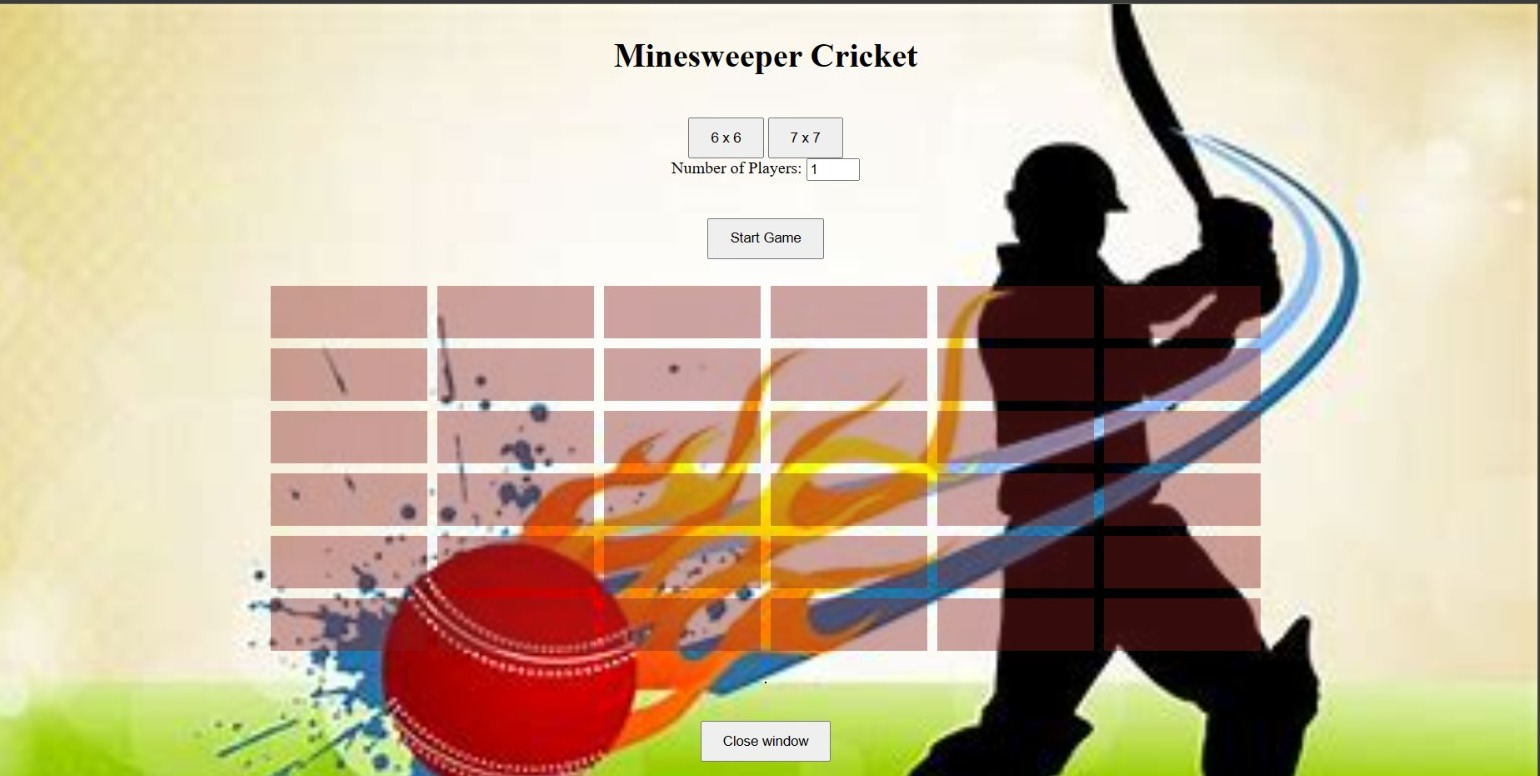
\includegraphics[width=0.5\textwidth]{basic page.jpeg}
    \caption{Basic page}
    \label{fig:basic}
\end{figure}

\begin{figure}[h!]
    \centering
    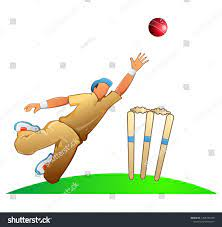
\includegraphics[width=0.2\textwidth]{fielder.jpeg}
    \caption{Fielder}
    \label{fig:fielder}
\end{figure}

\section{How to play}
Initially, the player has to choose the number of grids in which he/she wants to play, and if more number of people want to play, they can choose the number of players. Start button has to be clicked to start the game.\\
For a single player, the current score is displayed at the bottom and once the game is over, fielders in the grids become visible with an animation poping on the centre of the screen saying out. Final score is displayed at the bottom.\\
Multiplayer rules are explained as part of Customisation \ref{mul}.




\section{Customization}


\subsection{Choosing Grid Size}
The player can choose between a 6x6 and a 7x7 grid in the beginning of the game. This is done using a button. The grid is generated accordingly.

\subsection{Runs in each grid}
Each grid has some random number hidden behind it. These are either 1,2,3,4, or 6 runs, each with a specific frequency of appearance.



\subsection{Multiplayer Player Mode}
\label{mul}

If more than one player wishes to play, they can do so by changing the number of players input. Maximum of 7 players can play at a time. Their current scores and their status (whether they got out or not) are displayed in a table.
Each person gets their chances of play one after the another and once they get out, they can't play anymore. Whoever scores the maximum score wins the match.

\subsection{Styling}
The page is styled using external CSS. The background image is a cricketer animation on which the grids are kept at the center of the screen.
Once a player gets out, an animation pops up in the center of the screen(see \fig[\ref{fig:animation}]). For multiple players, the scores of each player are displayed as a table.\\
Once the player gets out, fielders in the grid are revealed.\\
Finally, the winner player is displayed. 
\begin{figure}[h!]
    \centering
    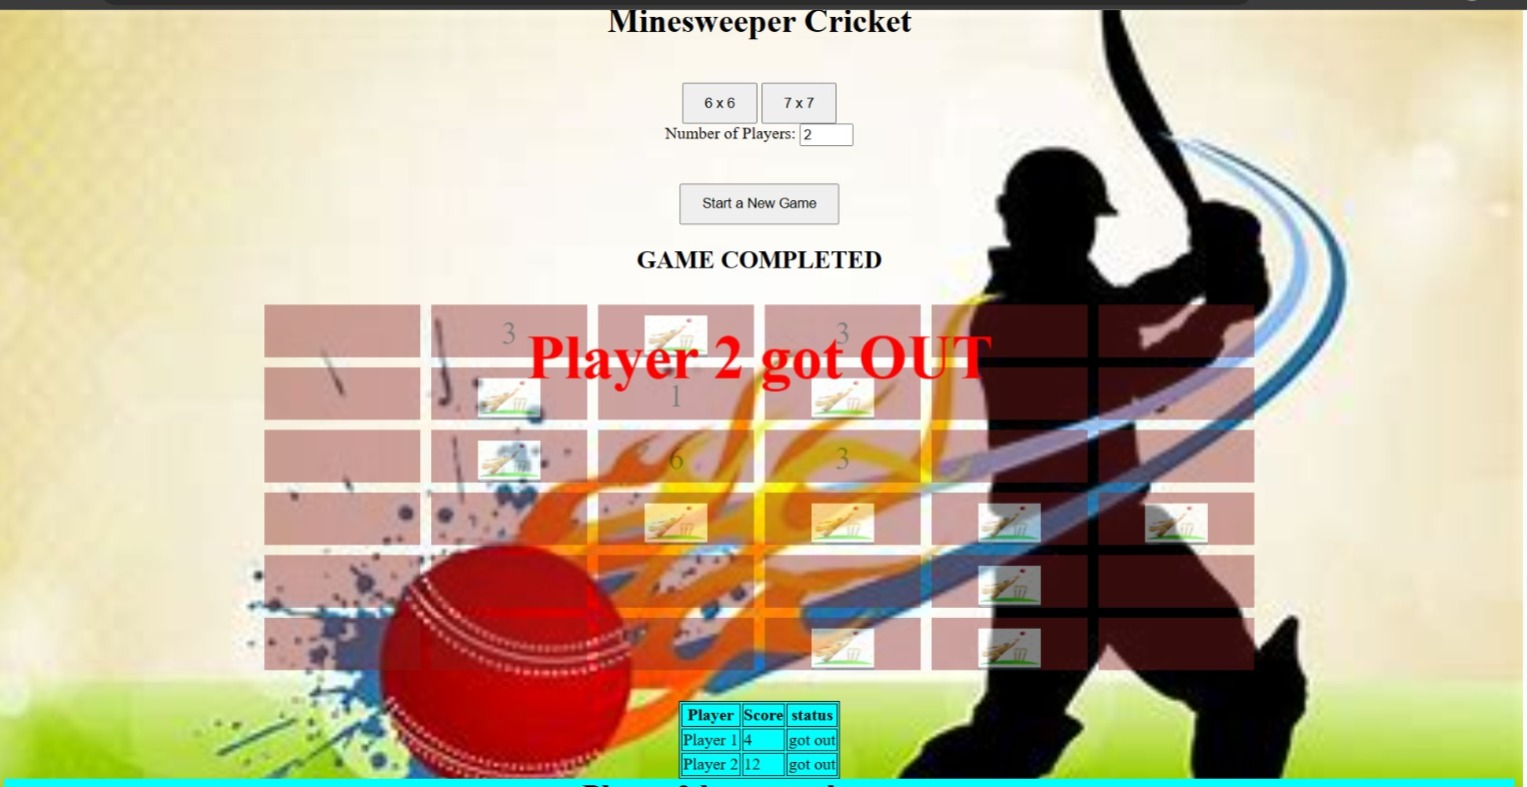
\includegraphics[width=0.5\textwidth]{animation.jpg}
    \caption{Basic page}
    \label{fig:animation}
\end{figure}

\subsection{Close Window}
This button closes the window.
\subsection{Removing Glitches}
Once the game is started, to avoid clicking of any of the settings, The buttons grey out, and will be disabled. Once the game is over, they return to normal.
Even if the same grid is clicked twice, the grid is not clicked twice and remains inactive.

\section{Code Structure}

I used many functions to represent my code more readable. Understandable names are given to it functions which are self explanatory, eg- game\_start, game\_middle, etc.\\
There are mainly two types of functions. One set are for single player mode and other set are for multiplayer mode.\\
Once the game is started, fielders and scores are randomly placed hidden behind every grid and if a grid is clicked , game\_middle function is called. If a fielder button is clicked, game\_end button is called.

\section{References}

\url{https://www.w3schools.com/html/html_css.asp} - used for css styling\\
\url{https://www.w3schools.com/css/css_grid.asp} - used for creating grids


\end{document}
